% Ubah kalimat sesuai dengan judul dari bab ini
\chapter{PENGUJIAN DAN EVALUASI}

Bab ini membahas skenario pengujian yang dilakukan untuk memvalidasi kinerja sistem serta hasil evaluasi dari modul klasifikasi dan modul koreksi. Pengujian bertujuan untuk memastikan bahwa model yang dibangun mampu mengenali jenis artefak dengan akurat dan memperbaiki citra yang rusak secara efektif.

\section{Skenario Pengujian}

Skenario pengujian dirancang untuk mengukur kinerja model dalam lingkungan yang terkontrol namun representatif terhadap masalah yang dihadapi. Pengujian dilakukan secara terpisah untuk modul klasifikasi dan modul koreksi.

\subsection{Lingkungan Pengujian}

Seluruh proses pelatihan dan pengujian dilakukan menggunakan platform Kaggle Notebook. Lingkungan ini menyediakan spesifikasi perangkat keras berupa satu GPU NVIDIA Tesla P100 dan RAM sebesar 32 GB yang memadai untuk komputasi \textit{deep learning}. Perangkat lunak utama yang digunakan adalah bahasa pemrograman Python 3.10 dengan dukungan \textit{library} Tensorflow, Pytorch, Transformers, Pandas, NumPy, dan Matplotlib. 

\subsection{Skenario Pengujian Modul Klasifikasi}

Pengujian modul klasifikasi bertujuan membandingkan performa antara arsitektur CNN dan Transformer. Dalam pelaksanaannya, dataset dibagi menjadi data latih (\textit{training set}) yang digunakan untuk melatih bobot model dan data uji (\textit{test set}) yang digunakan sebagai data validasi untuk memantau metrik performa seperti \textit{validation loss} dan akurasi pada setiap epoch. Data uji juga digunakan sebagai acuan dalam penerapan mekanisme \textit{early stopping} untuk mencegah terjadinya \textit{overfitting}.

Konfigurasi \textit{hyperparameter} ditetapkan secara seragam pada aspek-aspek umum untuk memastikan perbandingan yang adil antara model CNN (ResNet50, DenseNet121, EfficientNetB0) dan Transformer (ViT, Swin Transformer). Meskipun demikian, penyesuaian khusus tetap dilakukan pada komponen \textit{optimizer} dan regularisasi agar kinerja masing-masing arsitektur dapat mencapai titik optimal. Rincian lengkap mengenai konfigurasi tersebut disajikan pada Tabel \ref{tb:hyperparameter}

%Inout tabel hyperaparameter
% Contoh pembuatan tabel
\begin{longtable}{|p{2cm}|p{4cm}|p{4cm}|}
  % Keterangan dari tabel yang dibuat
  \caption{Konfigurasi \textit{Hyperparameter} Model Klasifikasi}
  % Label referensi dari tabel yang dibuat
  \label{tb:hyperparameter}\\
  % Isi dari tabel yang dibuat
  \hline
  \rowcolor[HTML]{C0C0C0}
  \textbf{Parameter} & \textbf{Konfigurasi CNN} & \textbf{Konfigurasi Transformer} \\ \hline
  \textit{Input Size} & ResNet \& DenseNet: $256 \times 256$, EfficientNet: $224 \times 224$ & SwinV2: $224 \times 224$, ViT: $256 \times 256$ \\ \hline
  \textit{Batch Size} & 32 & 32 \\ \hline
  \textit{Optimizer} & Adam & AdamW \\ \hline
  \textit{Learning Rate} & \textit{Warm Up}:$1e-4$, \textit{Fine tune}: $7e-6$ & $1e-4$ \\ \hline
  Epochs & \textit{Warm Up}: 10, \textit{Fine Tune}: 40 & 20 \\ \hline
  Regularisasi & \textit{Dropout (0.5)}, \textit{Early Stopping (Patience=5)}& \textit{Weight Decay (0.01), Early Stopping (Patience=5)} \\ \hline
  Augmentasi & \textit{RandomFlip, RandomZoom} & \textit{RandomFlip, ColorJitter, RandomResizedCrop} \\ \hline
\end{longtable}
 

Setelah proses pelatihan selesai, kinerja model dievaluasi secara menggunakan empat metrik klasifikasi utama. Akurasi (\textit{Accuracy}) digunakan untuk melihat rasio prediksi yang benar terhadap keseluruhan data. Presisi (\textit{Precision}) dihitung untuk mengukur ketepatan prediksi positif model terhadap data aktual, yang sangat penting untuk meminimalkan \textit{false positive}. \textit{Recall} (sensitivitas) digunakan untuk mengukur kemampuan model dalam menemukan kembali seluruh informasi yang relevan. Terakhir, F1-Score digunakan sebagai rata-rata harmonik antara presisi dan \textit{recall} untuk memberikan gambaran kinerja yang seimbang pada dataset \textit{multi-class}.

\subsection{Skenario Pengujian Modul Koreksi}

Pengujian modul koreksi difokuskan untuk menilai kemampuan \textit{Generator} dalam arsitektur Pix2Pix GAN untuk merekonstruksi citra bersih dari citra dengan artefak. Model dilatih dengan input citra berukuran $256 \times 256$ piksel selama 250 epoch. Proses optimasi menggunakan algoritma Adam dengan parameter momentum $\beta_1=0.5$ dan $\beta_2=0.999$, serta learning rate konstan sebesar $2e-4$. Dalam fungsi \textit{loss} gabungan, bobot $\lambda$ diatur sebesar 100. Nilai ini dipilih untuk memberikan prioritas yang jauh lebih tinggi pada L1 \textit{Loss} (kemiripan piksel absolut) dibandingkan \textit{Adversarial Loss}. Tujuannya adalah memastikan struktur anatomi otak tetap terjaga dan tidak berubah bentuk meskipun teksturnya diperbaiki oleh GAN.

Kualitas citra hasil rekonstruksi kemudian dievaluasi menggunakan dua metrik standar dalam pemrosesan citra medis. Metrik pertama adalah \textit{Peak Signal-to-Noise Ratio} (PSNR) yang mengukur rasio antara nilai maksimum sinyal dan noise dalam satuan desibel (dB); nilai yang lebih tinggi mengindikasikan kualitas rekonstruksi yang lebih baik. Metrik kedua adalah \textit{Structural Similarity Index} (SSIM) yang mengukur kemiripan struktural (luminansi, kontras, dan struktur) antara citra hasil koreksi dengan citra asli (\textit{ground truth}). Nilai SSIM berkisar antara -1 hingga 1. Nilai yang mendekati 1 menunjukkan bahwa struktur citra hasil rekonstruksi sangat identik dengan aslinya.

\section{Evaluasi Pengujian}

Bagian ini memaparkan hasil eksperimen berdasarkan skenario yang telah ditetapkan di atas, mencakup analisis kuantitatif dan kualitatif.

\subsection{Evaluasi Modul Klasifikasi Artefak}

Berdasarkan pelatihan yang dilakukan pada lima model berbeda, diperoleh hasil evaluasi kuantitatif pada data uji. Rangkuman mengenai metrik terbaik yang dicapai oleh masing-masing model ditunjukkan pada Tabel \ref{tb:classificationperf}.

% Gunakan environment 'table' dengan opsi [H] agar tabel tidak terpotong
\begin{table}[H]
	\centering
	\caption{Perbandingan Kinerja Metrik Model Klasifikasi}
	\label{tb:classificationperf}
	
	\vspace{2ex}
	
	% Gunakan tabularx agar lebar pas \textwidth
	% X = Kolom fleksibel (rata kiri, auto wrap)
	% c = Kolom tengah (centered) untuk angka
	\begin{tabularx}{\textwidth}{|X|c|c|c|c|}
		\hline
		\rowcolor[HTML]{C0C0C0}
		\textbf{Model} & \textbf{Akurasi} & \textbf{Presisi} & \textbf{\textit{Recall}} & \textbf{\textit{F1-Score}} \\ \hline
		
		\textbf{ResNet50} & 0.8890 & 0.9053 & 0.8890 & 0.8908 \\ \hline
		\textbf{DenseNet121} & 0.9031 & 0.9106 & 0.9031 & 0.9035 \\ \hline
		\textbf{EfficientNetB0} & 0.8469 & 0.8586 & 0.8469 & 0.8490 \\ \hline
		\textbf{ViT} & 0.8876 & 0.8923 & 0.8876 & 0.8881 \\ \hline
		\textbf{SwinV2 Transformer} & 0.9382 & 0.9539 & 0.9537 & 0.9536 \\ \hline
		
	\end{tabularx}
\end{table}

Analisis hasil menunjukkan bahwa model SwinV2 Transformer mencapai kinerja tertinggi secara konsisten di semua metrik dengan akurasi 93.82\% dan F1-Score 95.36\%. Keunggulan yang signifikan ini disebabkan oleh mekanisme \textit{shifted window attention} yang efektif menangkap konteks lokal maupun global pada citra artefak.

Pada model berbasis CNN, DenseNet menunjukkan kinerja yang paling tinggi dengan akurasi 90.31\% mengungguli ResNet (88.90\%). Hal ini menunjukkan bahwa \textit{dense connections} pada DenseNet membantu dalam propagasi fitur yang lebih efisien dibandingkan \textit{residual connections} pada ResNet untuk tugas klasifikasi ini. Namun, secara keseluruhan, arsitektur Transformer menunjukkan potensi yang lebih besar dengan SwinV2 Transformer secara signifikan mengungguli model-model lainnya.

\begin{figure}[H]
	\centering
	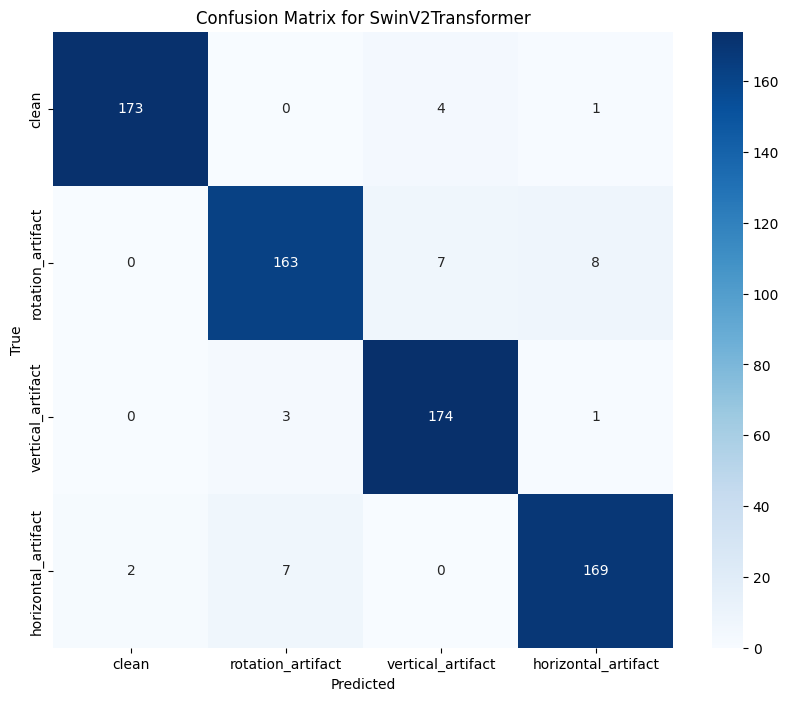
\includegraphics[width=0.9\linewidth]{gambar/swinv2-confusionmatrix.png}
	\caption{\textit{Confusion Matrix} Model Terbaik (SwinV2 Transformer)}
	\label{fig:confusionmatrixswinv2}
\end{figure}


Analisis lebih mendalam dilakukan menggunakan \textit{Confusion Matrix} pada model terbaik (SwinV2 Transformer) yang ditunjukkan pada Gambar \ref{fig:confusionmatrixswinv2} untuk memahami karakteristik prediksi model secara spesifik pada tiap kelas.

\begin{sloppypar}
	Analisis lebih mendalam terhadap Confusion Matrix pada model SwinV2 Transformer menunjukkan karakteristik prediksi yang sangat kuat dalam membedakan citra bersih dari citra dengan artefak. Namun, terdapat pola misklasifikasi yang spesifik jika ditinjau antar kategori artefak. Kesalahan prediksi paling signifikan terjadi pada diferensiasi antara artefak horizontal dengan artefak rotasi, dilanjutkan oleh kesalahan dalam membedakan artefak vertikal dengan artefak rotasi. Selain itu, terdapat pula kecenderungan model salah mengklasifikasikan artefak rotasi sebagai artefak horizontal, dengan frekuensi tertinggi mencapai 8 sampel pada kategori tersebut. Fenomena ini mengindikasikan bahwa pada irisan otak tertentu, distorsi spasial yang dihasilkan oleh gerakan rotasi memiliki kemiripan fitur tekstur dengan pola \textit{ghosting} atau \textit{blurring} linear yang dihasilkan oleh gerakan translasi secara horizontal maupun vertikal. Hal ini menyebabkan batas keputusan model menjadi sedikit samar di antara jenis-jenis gerakan tersebut.
\end{sloppypar}

\subsection{Evaluasi Modul Koreksi Citra}

Pengujian modul koreksi dilakukan dengan membandingkan citra berartefak dan citra hasil restorasi \textit{Generator} terhadap citra asli untuk melihat seberapa baik kemiripan citra yang  dikoreksi dengan citra aslinya jika dibandingkan dengan citra berartefak. Hasil evaluasi dari 200 sampel gambar tes ditunjukkan pada Tabel \ref{tb:gan-perf}. 

% Gunakan environment 'table' dengan opsi [H] agar tabel tidak terpotong
\begin{table}[H]
	\centering
	\caption{Perbandingan Kinerja Metrik Model Klasifikasi}
	\label{tb:gan-perf}
	
	\vspace{2ex}
	
	% Gunakan tabularx agar lebar pas \textwidth
	% X = Kolom fleksibel (rata kiri, auto wrap)
	% c = Kolom tengah (centered) untuk angka
	\begin{tabularx}{\textwidth}{|X|c|c|c|}
		\hline
		\rowcolor[HTML]{C0C0C0}
		\textbf{Metrik} & \textbf{Gambar Berartefak} & \textbf{Gambar Koreksi} & \textbf{Perbedaan}\\ \hline
		
		\textbf{PSNR} & 34.3287 dB & 32.8180 dB & -1.5107  \\ \hline
		\textbf{SSIM} & 0.9061 & 0.9099 & +0.0038 \\ \hline
	\end{tabularx}
\end{table}

Berdasarkan tabel evaluasi kuantitatif, hasil pengujian menunjukkan peningkatan nilai SSIM pada gambar hasil koreksi dibandingkan dengan baseline gambar berartefak. Peningkatan ini mengindikasikan bahwa model GAN berhasil merestorasi integritas struktural dan geometri anatomis citra medis, sehingga \textit{motion artifact} yang mengganggu visualisasi berhasil direduksi. Sebaliknya, nilai PSNR mengalami penurunan setelah dilakukan koreksi. Penurunan ini menunjukkan bahwa meskipun kualitas visual membaik, terdapat deviasi pada intensitas piksel absolut yang kemungkinan disebabkan oleh \textit{micro-texture generation} atau pergeseran piksel minor yang dilakukan oleh generator untuk meningkatkan ketajaman gambar. Hasil ini menegaskan bahwa model lebih berfokus pada kualitas kemiripan struktur gambar dibandingkan dengan kualitas akurasi pada level piksel.


\begin{figure}[H]
	\centering
	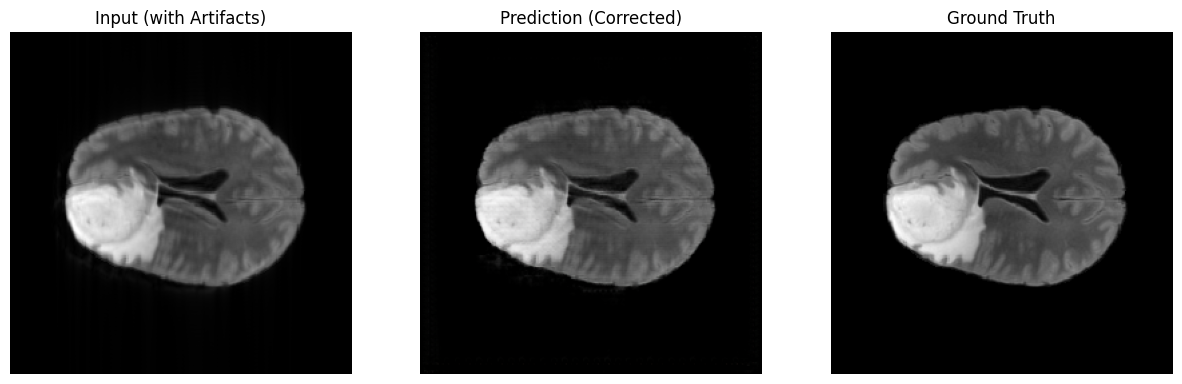
\includegraphics[width=\linewidth]{gambar/gan-image-correction.png}
	\caption{Perbandingan Visual Hasil Koreksi Citra MRI}
	\label{fig:ganimagecompare}
\end{figure}

Secara kualitatif, Gambar \ref{fig:ganimagecompare} menunjukkan kemampuan model dalam meningkatkan ketajaman visual citra yang semula kabur akibat artefak \textit{ghosting}. Alih-alih sekadar mencocokkan intensitas piksel, \textit{Generator} berfokus pada rekonstruksi tekstur dan tepi organ agar terlihat realistis. Hasilnya adalah area latar belakang menjadi lebih bersih dan garis-garis anatomis otak terlihat jauh lebih terlihat dibandingkan citra input. Peningkatan kualitas visual ini mengindikasikan bahwa model memprioritaskan pemulihan fitur-fitur penting yang diperlukan untuk interpretasi visual, meskipun secara statistik terdapat penurunan intensitas sinyal absolut.
